\documentclass[9pt,a4paper]{article}

% ---- Strong compact layout (single column) ----
\usepackage[a4paper,margin=0.5cm]{geometry}
\usepackage[T1]{fontenc}
\usepackage{lmodern}
\usepackage[expansion=false]{microtype}

\usepackage{titlesec}
\titlespacing*{\section}{0pt}{*1.0}{*0.4}
\titlespacing*{\subsection}{0pt}{*0.8}{*0.3}
\titlespacing*{\subsubsection}{0pt}{*0.7}{*0.2}

\usepackage{enumitem}
\setlist{itemsep=1pt, topsep=3pt}

\setlength{\parskip}{2pt}
\setlength{\parindent}{0pt}

\usepackage[T1]{fontenc}
\usepackage{amsmath}
\usepackage{amssymb}
\usepackage{braket}
\usepackage{amsfonts} % oder amssymb
\usepackage{graphicx}

\linespread{0.95}
\begin{document}
    \tableofcontents
    \section{Komplexe Zahlen}
    \subsection{Grundlagen - Imaginäre Einheit}
    $$z^2 + 1 = 0$$
    $$z^2 = -1$$
    $$nicht möglich\implies	 x^2 \ge 0$$
    $$i^2 = -1$$
    
    \subsection{Grundlagen - Format Komplexe Zaheln}
    Jede Komplexe zahl $z \in \mathbb{C}$ hat einen Realanteil und einen Imaginaranteil:
    $$z=x+yi \implies x,y \in \mathbb{R}$$
    
    \subsection{Grundlagen - Menge der komplexen Zahlen}
    
    $$ \mathbb{C} := \{z| z=x +yi, x,y \in \mathbb{R}, i^2 = -1\}$$
    
    \subsection{Grundlagen - Die Komplexe Zahlenebene}
    
    Die reellen Zahlen k¨onnen auf einer Geraden dargestellt werden, der reellen Zahlengerade. Eine komplexe
    Zahl $z=x+yi \in \mathbb{C}$ ist durch zwei reelle Zahlen x und y eindeutig bestimmt. Diese beiden reellen Zahlen
    können als Punkt $(x|y)$ oder als Vektor $\begin{pmatrix} x \\ y \end{pmatrix}$ in einer Ebene dargestellt werden. Diese Ebene heisst **komplexe Zahlenebene** oder **Gaussche Ebene**.
    
    Sei $z=x+yi \in \mathbb{C}$ eine komplexe Zahl. Dann bezeichnet.
    $$Re(z):=x$$
    den Realteil
    $$Im(z):=y$$
    den Imaginärteil
    
    Für Komplexe Zahlen gilt:
    $$Re(z)=\frac{z+=z}{2}$$
    $$Im(z)=\frac{z-=z}{2}$$
    $$z==z z \in$$
    $$\overline{\overline{z}}=z$$
    $$\overline{z+w}=\overline{z}+\overline{w}$$
    $$\overline{z+w}=\overline{z}*\overline{w}$$
    $$\overline{\frac{1}{z}}=\frac{1}{\overline{z}}$$
    
    \subsection{Addition / Subtraktion}
    $$z_1\pm z_2=(a_1+b_1*i)\pm(a_2+b_2*i)$$
    \subsubsection{Additon}
    $$=(a_1+a_2)+(b_1+b_2)*i$$
    \subsubsection{Subtraktion}
    $$=(a_1-a_2)+(b_1-b_2)*i$$
    
    \subsubsection{Multiplikation}
    $$z_1*z_2=(a_1*a_2-b_1*b_2)+(a_1*b_2+a_2*b_1)*i$$
    
    \subsubsection{Division}
    \paragraph{Division in kartesischer Form}\mbox{}\\
    
    Für \[
    z_1 = a+bi,\qquad z_2 = c+di \neq 0
    \]
    gilt durch Multiplizieren mit dem konjugierten Nenner:
    \[
    \frac{a+bi}{c+di}
    =
    \frac{(a+bi)(c-di)}{c^2+d^2}
    =
    \frac{ac+bd}{c^2+d^2}
    +
    i\,\frac{bc-ad}{c^2+d^2}.
    \]
    
    Dabei ist
    \[
    c^2+d^2 = |z_2|^2.
    \]
    
    \paragraph{Division in Polar-/Exponentialform}\mbox{}\\
    
    Für
    \[
    z_1 = r_1(\cos\varphi_1+i\sin\varphi_1), \qquad
    z_2 = r_2(\cos\varphi_2+i\sin\varphi_2)
    \]
    gilt:
    \[
    \frac{z_1}{z_2}
    =
    \frac{r_1}{r_2}
    \Big(\cos(\varphi_1-\varphi_2)+i\sin(\varphi_1-\varphi_2)\Big).
    \]
    
    % ---------- Merksatz ----------
    \[
    \text{Beträge dividieren, Winkel subtrahieren.}
    \]
    
    \subsection{Komplexe Konjugierte}
    $$z=x+yi$$
    $$={z}=x-yi$$
    
    \subsection{Absolutbetrag}
    $$r=\vert z \vert=\sqrt{(x^2+y^2)}=\sqrt{z\overline{z}}$$
    $$r=\vert z \vert=\sqrt{(Re(z)^2+Im(z)^2)}$$
    $$|z|^2=z\overline{z}$$
    
    \subsection{Periodizität von Komplexen Zahlen}
    $$i^0=1,i^1=i,i^2=-1,i^3=-i,i^4=1 (und wiederholt sich).$$
    Die Formel lautet für $n=exponent$:
    $$n\ mod \ 4 = k => i^k$$
    **Beispiel:**
    $$50 mod 4=2i^{50}=i^2=-1.$$
    \subsection{Polarform}
    \subsubsection{trigonometrische Form}
    $$z=r(cos(\phi)+i*sin(\phi)$$
    $$z=r*cis(\phi)$$
    
    \subsubsection{Umrechnung Polarform zu kartesische Form}
    $$x = r*cos(\phi)$$
    $$y = r*sin(\phi)$$
    \subsubsection{Umrechnung kartesische Form zu Polarform}
    \paragraph{Argument}
    Eine komplexe Zahl besitzt unendlich viele Argumente:
    \[
    \varphi + 2k\pi,\qquad k\in\mathbb{Z}.
    \]
    
    Um einen eindeutigen Winkel zu erhalten, definiert man den Hauptwert:
    \[
    \arg(z)\in(-\pi,\pi].
    \]
    
    Dieser Bereich deckt den Einheitskreis genau einmal ab; dabei ist
    \(\pi\) enthalten und \(-\pi\) ausgeschlossen, damit es keine
    Doppelwerte auf der negativen x-Achse gibt.
    
    \[
    \varphi =
    \begin{cases}
        \arctan\left(\dfrac{y}{x}\right), & x > 0 \\[1em]
        \arctan\left(\dfrac{y}{x}\right) + \pi, & x < 0,\; y \ge 0 \\[1em]
        \arctan\left(\dfrac{y}{x}\right) - \pi, & x < 0,\; y < 0 \\[1em]
        \frac{\pi}{2}, & x = 0,\; y > 0 \\[0.5em]
        -\frac{\pi}{2}, & x = 0,\; y < 0
    \end{cases}
    \]
    
    
    \subsection{Exponentialform}
    
    \subsubsection{Eulerformel}
    \[
    e^{it} = \cos(t) + i\sin(t)
    \]
    
    \subsubsection{Beziehungen für Sinus und Cosinus}
    \[
    \cos(t)=\frac{e^{it}+e^{-it}}{2}
    \]
    \[
    \sin(t)=\frac{e^{it}-e^{-it}}{2i}
    \]
    
    \subsubsection{Allgemeine komplexe Exponentialfunktion}
    \[
    e^z = e^{\sigma+it}=e^\sigma(\cos(t)+i\sin(t))
    \]
    
    \subsubsection{Darstellungen komplexer Zahlen}
    \[
    z = x + iy
    \]
    \[
    z = r(\cos(\varphi)+i\sin(\varphi))
    \]
    \[
    z = re^{i\varphi + k\cdot 2\pi i}, \quad k\in\mathbb{Z}
    \]
    
    \subsubsection{Umrechnung}
    \[
    r = |z| = \sqrt{x^2+y^2}
    \]
    \[
    \varphi = \arg(z)\in(-\pi,\pi)
    \]
    
    \subsubsection{Komplexer Logarithmus}
    Für $z \neq 0$ in Polarform
    \[
    z = re^{i\varphi}, \quad r = |z|, \;\varphi = \arg(z)
    \]
    ist der mehrwertige Logarithmus definiert als
    \[
    \log z = \ln r + i(\varphi + 2\pi k), \quad k \in \mathbb{Z}.
    \]
    
    \textbf{Hauptwert:}
    \[
    \operatorname{Log}z = \ln r + i\,\arg(z), \qquad -\pi < \arg(z)\le \pi.
    \]
    
    
    \subsubsection{Komplexe Wurzeln}
    Gesucht sind Lösungen von
    \[
    z^n = w.
    \]
    Schreibe $w$ in Polarform
    \[
    w = Re^{i\theta}.
    \]
    Dann sind alle Lösungen
    \[
    z_k = \sqrt[n]{R}\, e^{i\frac{\theta + 2\pi k}{n}}, \qquad k=0,\dots,n-1.
    \]
    Es gibt also $n$ verschiedene Lösungen, die gleichmäßig auf einem Kreis liegen.
    
    
    \subsubsection{Komplexe Potenzen}
    Für eine komplexe Potenz gilt
    \[
    z^a = e^{a\log z}.
    \]
    Da $\log z$ mehrdeutig ist,
    \[
    z^a = e^{a(\ln r + i(\varphi + 2\pi k))}, \qquad k\in\mathbb{Z}.
    \]
    Im Allgemeinen existieren also unendlich viele Werte.
    Verwendet man den Hauptwert,
    \[
    z^a = e^{a\operatorname{Log}z}.
    \]
    
    
    \subsubsection{Typische Gleichungen}
    
    \paragraph{1. Gleichungen der Form $z^n = w$:}
    \[
    z_k = \sqrt[n]{R}\, e^{i\frac{\theta + 2\pi k}{n}}, \qquad k=0,\dots,n-1.
    \]
    
    \paragraph{2. Exponentialgleichungen $e^z = w$:}
    Schreibe $w = Re^{i\theta}$, dann
    \[
    z = \ln R + i(\theta + 2\pi k), \qquad k\in\mathbb{Z}.
    \]
    
    \paragraph{3. Gleichungen $z^a = b$:}
    \[
    z^a = b \Rightarrow a\log z = \log b,
    \]
    Mehrdeutigkeit über $2\pi k$ berücksichtigen und nach $z$ lösen.
    
    
    \subsubsection{Lösestrategie}
    \begin{enumerate}
        \item Schreibe komplexe Zahlen in Polarform: $z = re^{i\varphi}$.
        \item Logarithmus korrekt verwenden: $\log z = \ln r + i(\varphi + 2\pi k)$.
        \item Potenzen als Exponentialfunktion: $z^a = e^{a\log z}$.
        \item Real- und Imaginärteile vergleichen.
        \item Alle $k$ berücksichtigen $\Rightarrow$ mehrere Lösungen.
    \end{enumerate}
    
    \section{Lineare Algebra}
    \subsection{Vektoren}
    $$\Theta = \arctan(\frac{y}{x})$$
    \subsection{Länge einer Vektors (Betrag)}
    
    Für einen Vektor 
    \[
    \vec{v} = (v_1, v_2, \dots, v_n)
    \]
    ist der Betrag (die Länge, Norm)
    \[
    |\vec{v}| = \sqrt{v_1^2 + v_2^2 + \dots + v_n^2}.
    \]
    
    \subsection*{Spezialfälle}
    Im $\mathbb{R}^2$:
    \[
    \vec{v}=(x,y) \quad\Rightarrow\quad |\vec{v}|=\sqrt{x^2+y^2}
    \]
    
    Im $\mathbb{R}^3$:
    \[
    \vec{v}=(x,y,z) \quad\Rightarrow\quad |\vec{v}|=\sqrt{x^2+y^2+z^2}
    \]
    
    \subsection*{Eigenschaften}
    \[
    |\vec{v}| \ge 0,\qquad
    |\vec{v}| = 0 \Leftrightarrow \vec{v} = \vec{0},\qquad
    |k\vec{v}| = |k|\cdot|\vec{v}|
    \]
    Dreiecksungleichung:
    \[
    |\vec{a}+\vec{b}| \le |\vec{a}| + |\vec{b}|
    \]
    
    
    \subsection{Vektoraddition}
    $$\begin{bmatrix} x_1 \\ y_1 \end{bmatrix} + \begin{bmatrix} x_2 \\ y_2 \end{bmatrix} = \begin{bmatrix} x_1 + x_2 \\ y_1 + y_2\end{bmatrix}$$
    \subsection{Vektorsubtraktion}
    $$\begin{bmatrix} x_1 \\ y_1 \end{bmatrix} - \begin{bmatrix} x_2 \\ y_2 \end{bmatrix} = \begin{bmatrix} x_1 - x_2 \\ y_1 - y_2\end{bmatrix}$$
    \subsection{Norm eines Vektors (Länge)}
    Generel für $\mathbb{C}$ und  $\mathbb{R}$
    $$\sqrt{\sum_{i=1}^n |x_i|^2} =\sqrt{|x_1|^2+|x_2|^2...+|x_n|^2}$$
    Beispiel Reell
    im Reelen braucht es die Beträge nicht:
    $$||x|| = \sqrt{{x_1}^2+{x_2}^2 ... + {x_n}^2}$$
    $$a=\begin{bmatrix}
        a_{1} \\
        a_{2}
    \end{bmatrix}; ||a|| = \sqrt{{a_1}^2+{a_2}^2} $$
    Beispiel Komplex
    $$||z|| = \sqrt{{|z_1|}^2+{|z_2|}^2 ... + {|z_n|}^2}$$
    $$a=\begin{bmatrix}
        2+i \\
        2-i
    \end{bmatrix}; ||a|| = \sqrt{|a_1|^2+|a_2|^2} $$
    \subsection{Skalare Multiplikation}
    $$\lambda * x = \lambda * \begin{bmatrix} x_1 \\ x_2 \end{bmatrix} = \begin{bmatrix} \lambda *x_1 \\ \lambda * x_2 \end{bmatrix}$$
    \subsection{Verbindungsvektor}
    $\overrightarrow{PQ}$ ist die symbolische Schreibweise für den Vektor mit Anfangspunkt $P$ und Endpunkt $Q$. Um Den Verbindungsvektor zu berechnen subtrahiert man den Fusspunkt (Subtrahend) von der Spitze (Minuend). Das gitl auch für Ortsvekoren anstatt Punkte.
    \[
    Q = \begin{bmatrix} x_Q \\ y_Q \end{bmatrix}
    \qquad
    P = \begin{bmatrix} x_P \\ y_P \end{bmatrix}
    \qquad
    \overrightarrow{PQ}
    = \begin{bmatrix} x_Q - x_P \\ y_Q - y_P \end{bmatrix}
    \]
    
    Es Gilt: $\overrightarrow{PQ}$ = $-\overrightarrow{QP}$
    
    \subsection{Parameterform Gerade}
    $$ \begin{bmatrix} x \\ y \\ z \end{bmatrix} = \begin{bmatrix} x _1 \\ y_2 \\ z_3 \end{bmatrix} + \lambda\begin{bmatrix} a_x \\ a_y \\ a_z \end{bmatrix} = $$
    
    Wobei  $\begin{bmatrix} x \\ y \\ z \end{bmatrix}$ den laufenden Punkte der Gerade bezeichnet, $\begin{bmatrix} x _1 \\ y_2 \\ z_3 \end{bmatrix}$ den Stützvektor und $\lambda\begin{bmatrix} a_x \\ a_y \\ a_z \end{bmatrix}$ den Richtungsvektor, wobei $\lambda$ die freie Variable, als Streckung vom Sütztvekotir darstellt.
    \subsection{Lineare Abhängigkeit}
    tbd
    
    \subsection{othogonale Projektion}
    Vektor b wird auf Vektor a projeziert
    \[
    \text{Proj}_{\vec{a}}(\vec{b}) 
    = \operatorname{proj}_{\vec{a}}(\vec{b})
    = \frac{\vec{a}\cdot\vec{b}}{|\vec{a}|^2}\,\vec{a}
    \]
    
    \[
    \left|\operatorname{proj}_{\vec{a}}(\vec{b})\right|
    = \frac{|\vec{a}\cdot\vec{b}|}{|\vec{a}|}
    \]
    
    
    \subsection{Skalarprodukt}
    Das Skalarprodukt ist folgendermassen definiert:
    $$\vec{a}*\vec{b}=\braket{a,b}=|\vec{a}||\vec{b}|\cos\sphericalangle(\theta)$$
    Für orthogonale Vektoren gilt folgendes
    
    \subsection{Berechnung Skalarprodukt}
    $$\overrightarrow{a} * \overrightarrow{b} = *\begin{bmatrix}a_x\\a_y\end{bmatrix} *\begin{bmatrix}b_x\\b_y\end{bmatrix} =
    (a_x b_x) + (a_yb_y)$$
    \subsection{Kreuzprodukt / Vektorprodukt}
    $$\overrightarrow{c}=\overrightarrow{a} \times \overrightarrow{b} $$
    1. $\overrightarrow{c}$ ist sowohl zu $\overrightarrow{a}$ als auch $\overrightarrow{b}$ othogonal.
    2. Der Betrag von $\overrightarrow{c}$ ist gleich dem Produkt aus den Beträgen der Vektoren $\overrightarrow{a}$ und $\overrightarrow{b}$ und dem Sinus des vonihnen eingeschlossenen Winkel $\phi$. Der Betrag von $\overrightarrow{c}$ entspricht dabei der Fläche eines Parallelogramms.
    
    Berechnung
    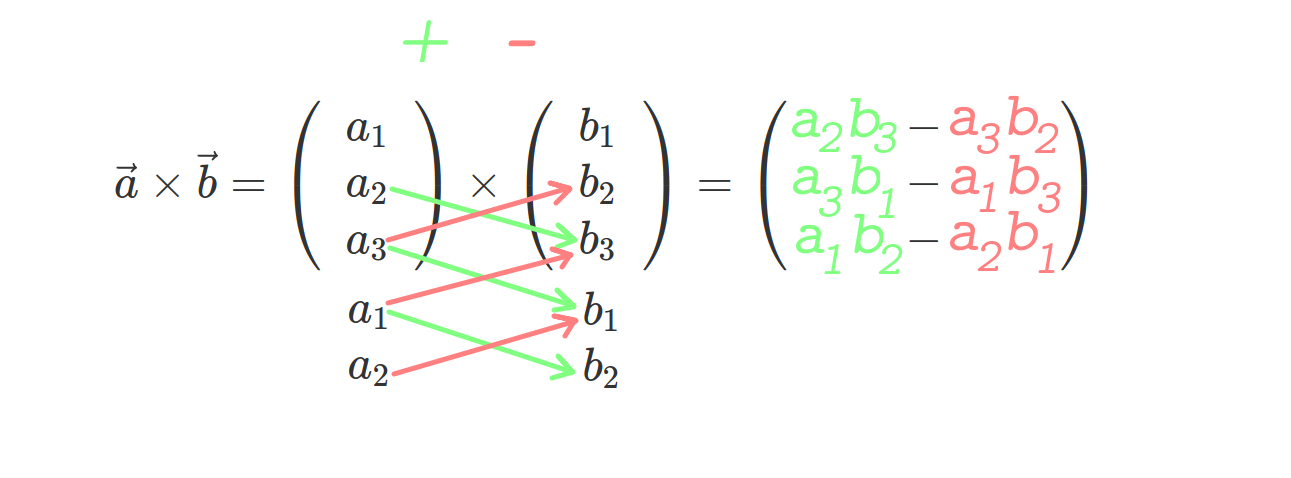
\includegraphics[width=1\linewidth]{img/kreuzprodukt}
    Projektion
    Seien $\overrightarrow{a}$ und $\overrightarrow{b}$ zwei  Vektoren  mit einem Winkel $\phi$ dazwischen. So berechnet man die Projektion von  $\overrightarrow{a}$ auf $\overrightarrow{b}$ folgendermassen.
    
    $\overrightarrow{b_a}=\frac{\braket{\overrightarrow{a},\overrightarrow{b}}}{{||\overrightarrow{a}||}^2}*\overrightarrow{a}$
    \subsection{Spatprodukt}
    Die Höhe eine spats ist folgendermassen definiert:
    $$h=||\overrightarrow{a}||*\cos{\phi}$$
    Die Fläche ist gleich dem Kreuzprodukt der Flächenvektoren:
    $A=|\overrightarrow{b}| \times |\overrightarrow{c}|$
    Das Volumen:
    $$V_{spat}=A*h=||\overrightarrow{b} \times \overrightarrow{c}||*||\overrightarrow{a}||*\cos{\phi}$$
    $$=|\braket{\overrightarrow{c},(\overrightarrow{a} \times \overrightarrow{b})}|$$
    \subsection{Tetraeder}
    Gegeben sind vier Punkte im Raum:
    $$A,B,C,D$$
    Dann bilden wir die drei Kantenvektoren, die von demselben Punkt ausgehen:
    $$\overrightarrow{a}=\overrightarrow{AB}, \overrightarrow{b}=\overrightarrow{AC}, \overrightarrow{c}=\overrightarrow{AD}$$
    Das Volumen V des Tetraeders ergibt sich zu:
    $$V=\frac{1}{6}\left| \overrightarrow{a}*(\overrightarrow{b}\times\overrightarrow{c})\right|$$
    Die Höhe h berechnet sich wie folgt:
    $$h = \frac{|\braket{\overrightarrow{c},(\overrightarrow{a} \times \overrightarrow{b})}|}{||(\overrightarrow{a} \times \overrightarrow{b})||}$$
    \subsection{Pyramide}
    Das Volumen der Pyrimafe aus den Fläachenpunkten: $A,B,C,D$ und den der Sptize $S$, berechnet sich wie folgt:
    $$V=\frac{1}{3}\left| \braket{(\overrightarrow{BA}\times\overrightarrow{BC}),\overrightarrow{BS}}\right|$$
    \section{Matrizen}
    Unter einer $m \times n$ - Matrix versteht man ein rechteckiges
    Zahlenschema von Zahlen $a_{ij} \in K$ mit $m$ Zeilen und $n$ Spalten:
    \subsection{Matrixaddition}
    Wenn Matrizen addiert werden, dann müssen beide Matrizen gleich gross sein:
    \[
    \mathbb{A}=
    \begin{pmatrix}
        a_{11} & a_{12} \\
        a_{21} & a_{22}
    \end{pmatrix}
    \qquad
    \mathbb{B}=
    \begin{pmatrix}
        b_{11} & b_{12} \\
        b_{21} & b_{22}
    \end{pmatrix}
    \qquad
    \mathbb{A}+\mathbb{B}=
    \begin{pmatrix}
        a_{11}+b_{11} & a_{12}+b_{12} \\
        a_{21}+b_{21} & a_{22}+b_{22}
    \end{pmatrix}
    \]
    
    \subsection{Matrixprodukt}
    Der Vektor muss gleich viele Einträge habe, wie die Matrix Spalten hat.
    \[
    y =
    \begin{pmatrix}
        y_{1} \\
        y_{2} \\
        y_{3}
    \end{pmatrix}
    =
    \begin{pmatrix}
        a_{11} & a_{12} & a_{13} \\
        a_{21} & a_{22} & a_{23} \\
        a_{31} & a_{32} & a_{33}
    \end{pmatrix}
    \begin{pmatrix}
        b_{1} \\
        b_{2} \\
        b_{3}
    \end{pmatrix}
    =
    \begin{pmatrix}
        a_{11}b_1 + a_{12}b_2 + a_{13}b_3 \\
        a_{21}b_1 + a_{22}b_2 + a_{23}b_3 \\
        a_{31}b_1 + a_{32}b_2 + a_{33}b_3
    \end{pmatrix}
    \]
    
    Produkt zweier Matrizen
    Das Produkt von zwei Matrizen funktioniert nur, wenn die erste Matriz gliech viele Spalte hat wie die die zweite Zeilen hat.
    \[
    \mathbb{Y} =
    \begin{pmatrix}
        a_{11} & a_{12} & a_{13} \\
        a_{21} & a_{22} & a_{23} \\
        a_{31} & a_{32} & a_{33}
    \end{pmatrix}
    \begin{pmatrix}
        b_{11} & b_{12} \\
        b_{21} & b_{22} \\
        b_{31} & b_{32}
    \end{pmatrix}
    =
    \begin{pmatrix}
        a_{11}b_{11} + a_{12}b_{21} + a_{13}b_{31} &
        a_{11}b_{12} + a_{12}b_{22} + a_{13}b_{32} \\
        a_{21}b_{11} + a_{22}b_{21} + a_{23}b_{31} &
        a_{21}b_{12} + a_{22}b_{22} + a_{23}b_{32} \\
        a_{31}b_{11} + a_{32}b_{21} + a_{33}b_{31} &
        a_{31}b_{12} + a_{32}b_{22} + a_{33}b_{32}
    \end{pmatrix}
    \]
    
    Matrixprodukte können alternativ auch mit dem Falkschem Schema berechnet werden. Das schafft ertwas meh Übericht beim rechnen. Siehe
    Transponierte Matrix
    Beim transponieren einer Matrix, werden die Zeilen zu Spalten.
    \[
    \mathbb{Y} =
    \begin{pmatrix}
        a_{11} & a_{12} & a_{13} \\
        a_{21} & a_{22} & a_{23} \\
        a_{31} & a_{32} & a_{33}
    \end{pmatrix}
    \qquad
    \mathbb{Y}^T =
    \begin{pmatrix}
        a_{11} & a_{21} & a_{31} \\
        a_{12} & a_{22} & a_{32} \\
        a_{13} & a_{23} & a_{33}
    \end{pmatrix}
    \]
    
    \subsection{Eigenwert einer Matrix}
    
    \subsection{Inverse Matrix}
    
    Eine Matrix $A$ heißt \textbf{invertierbar}, wenn eine Matrix $A^{-1}$ existiert mit
    \[
    A \cdot A^{-1} = A^{-1} \cdot A = I.
    \]
    
    Dies ist nur für quadratische Matrizen möglich.
    
    \subsubsection{Reguläre Matrix}
    Eine Matrix heißt \textbf{regulär} (oder \textbf{nicht-singulär}), wenn sie invertierbar ist.
    
    \[
    A \ \text{regulär} 
    \quad\Longleftrightarrow\quad
    \det(A) \neq 0
    \]
    
    Weitere äquivalente Bedingungen:
    \begin{itemize}
        \item $rang(A)=n$
        \item $A^{-1}$ existiert
        \item das LGS $Ax=b$ hat für jedes $b$ \textbf{genau eine} Lösung
    \end{itemize}
    
    \subsubsection{Singuläre Matrix}
    Eine Matrix heißt \textbf{singulär}, wenn sie nicht invertierbar ist.
    
    \[
    A \ \text{singulär}
    \quad\Longleftrightarrow\quad
    \det(A)=0
    \]
    
    Weitere Merkmale:
    \begin{itemize}
        \item $rang(A)<n$
        \item keine oder unendlich viele Lösungen für $Ax=b$
        \item der Kern ist nicht nur $\{0\}$
    \end{itemize}
    
    Determinante Uncleich 0 und rang gleich n
    \subsubsection{invertierbar}
    Sei $A \in \mathbb{R}^{n\times n}$. Dann sind äquivalent:
    
    \begin{itemize}
        \item $\det(A) \neq 0$
        \item $\operatorname{rang}(A) = n$
        \item Das lineare Gleichungssystem $Ax=b$ hat für jedes $b \in \mathbb{R}^n$ genau eine Lösung.
        \item $\ker(A) = \{0\}$
        \item $0$ ist kein Eigenwert von $A$.
        \item Es existiert eine Matrix $A^{-1}$ mit
        \[
        A A^{-1} = A^{-1} A = I.
        \]
    \end{itemize}
    \subsubsection{2x2 Matrix invertieren}
    Sei
    \[
    A =
    \begin{pmatrix}
        a & b\\
        c & d
    \end{pmatrix}
    \quad\text{mit}\quad
    \det(A)=ad-bc \neq 0.
    \]
    
    Dann ist
    \[
    A^{-1}
    =
    \frac{1}{ad-bc}
    \begin{pmatrix}
        d & -b\\
        -c & a
    \end{pmatrix}.
    \]
    
    \subsubsection{Matrix invertieren mit Gauß-Jordan}
    
    Eine Matrix $A$ ist invertierbar, wenn
    \[
    A^{-1}A = I.
    \]
    
    \paragraph*{Vorgehen}
    Zur Berechnung der Inversen stellt man die erweiterte Matrix
    \[
    [A \mid I]
    \]
    auf und führt Gauß--Jordan-Zeilenumformungen durch, bis links die
    Einheitsmatrix steht:
    \[
    [I \mid A^{-1}].
    \]
    
    Damit ergibt sich rechts automatisch die inverse Matrix $A^{-1}$.
    
    \paragraph*{Hinweise}
    \begin{itemize}
        \item nur quadratische Matrizen können invertierbar sein
        \item $A$ ist genau dann invertierbar, wenn $\det(A)\neq 0$
        \item erlaubt sind nur elementare Zeilenumformungen
    \end{itemize}
    
    \subsection{Spur (Trace) einer Matrix}
    
    \textbf{Definition:} Für eine quadratische Matrix
    \[
    A=\begin{pmatrix}
        a_{11} & a_{12} & \dots \\
        a_{21} & a_{22} & \dots \\
        \vdots & & \ddots
    \end{pmatrix}
    \]
    ist die Spur die Summe der Diagonalelemente:
    \[
    \mathrm{tr}(A)=\sum_{i=1}^{n} a_{ii}
    \]
    
    \textbf{Beispiel:}
    \[
    A=\begin{pmatrix}
        2 & 5\\
        -1 & 3
    \end{pmatrix}
    \qquad\Rightarrow\qquad
    \mathrm{tr}(A)=2+3=5
    \]
    
    \textbf{Eigenschaften:}
    \[
    \mathrm{tr}(A+B)=\mathrm{tr}(A)+\mathrm{tr}(B)
    \]
    \[
    \mathrm{tr}(cA)=c\,\mathrm{tr}(A)
    \]
    \[
    \mathrm{tr}(A)=\mathrm{tr}(A^T)
    \]
    \[
    \mathrm{tr}(AB)=\mathrm{tr}(BA)
    \]
    allgemeiner zyklisch:
    \[
    \mathrm{tr}(ABC)=\mathrm{tr}(BCA)=\mathrm{tr}(CAB)
    \]
    
    \textbf{Zusammenhang mit Eigenwerten:}
    \[
    \mathrm{tr}(A)=\lambda_1+\lambda_2+\dots+\lambda_n
    \]
    
    \textbf{Hinweis:} Die Spur ist nur für quadratische Matrizen definiert.
    
    \subsection{Arten von Matrizen}
    \subsubsection{Transponierte Matrix}
    
    Sei $A \in \mathbb{R}^{m \times n}$ mit
    \[
    A=\begin{pmatrix}
        a_{11}&a_{12}&\cdots&a_{1n}\\
        a_{21}&a_{22}&\cdots&a_{2n}\\
        \vdots&\vdots&\ddots&\vdots\\
        a_{m1}&a_{m2}&\cdots&a_{mn}
    \end{pmatrix}
    \qquad
    A^\top=\begin{pmatrix}
        a_{11}&a_{21}&\cdots&a_{m1}\\
        a_{12}&a_{22}&\cdots&a_{m2}\\
        \vdots&\vdots&\ddots&\vdots\\
        a_{1n}&a_{2n}&\cdots&a_{mn}
    \end{pmatrix}
    \]
    
    Die \textbf{transponierte Matrix} $A^\top \in \mathbb{R}^{n \times m}$ entsteht durch Vertauschen von Zeilen und Spalten:
    
    \paragraph*{Eigenschaften}
    \begin{itemize}
        \item $(A^\top)^\top = A$
        \item $(A + B)^\top = A^\top + B^\top$
        \item $(\lambda A)^\top = \lambda A^\top \quad (\lambda \in \mathbb{R})$
        \item $(AB)^\top = B^\top A^\top$
        \item Ist $A$ invertierbar: $(A^{-1})^\top = (A^\top)^{-1}$
    \end{itemize}
    
    \subsection*{Symmetrische Matrix}
    
    Eine Matrix $A \in \mathbb{R}^{n\times n}$ heißt symmetrisch, wenn
    \[
    A = A^{\mathsf T}.
    \]
    
    \paragraph{Eigenschaften:}
    \begin{itemize}
        \item Alle Eigenwerte sind reell.
        \item Eigenvektoren zu verschiedenen Eigenwerten sind orthogonal.
        \item Orthogonal diagonalisierbar: $A = Q D Q^{\mathsf T}$.
    \end{itemize}
    
    \subsection{Antisymmetrische Matrix}
    Eine Matrix $A \in \mathbb{R}^{n\times n}$ heißt antisymmetrisch, wenn
    \[
    A^{\mathsf T} = -A.
    \]
    
    \paragraph{Eigenschaften:}
    \begin{itemize}
        \item $a_{ii} = 0$ für alle $i$.
        \item Alle Eigenwerte sind rein imaginär oder $0$.
        \item Für alle $x \in \mathbb{R}^n$ gilt: $x^{\mathsf T} A x = 0$.
    \end{itemize}
    
    \subsubsection*{Hermitesche Matrix}
    
    Eine Matrix $A \in \mathbb{C}^{n\times n}$ heißt hermitesch, wenn
    \[
    A^{\mathsf *} = A,
    \]
    wobei $A^{\mathsf *} = \overline{A}^{\mathsf T}$.
    
    \paragraph{Eigenschaften}
    \begin{itemize}
        \item Alle Eigenwerte von $A$ sind reell.
        \item Eigenvektoren zu verschiedenen Eigenwerten sind orthogonal.
        \item $A$ ist unitär diagonalisierbar: $A = U D U^{\mathsf H}$.
    \end{itemize}
    
    \subsubsection*{Antihermitesche Matrix}
    
    Eine Matrix $A \in \mathbb{C}^{n\times n}$ heißt antihermitesch, wenn
    \[
    A^{\mathsf *} = -A,
    \]
    wobei $A^{\mathsf *} = \overline{A}^{\mathsf T}$.
    
    \paragraph*{Eigenschaften}
    \begin{itemize}
        \item Die Diagonaleinträge sind rein imaginär oder $0$.
        \item Alle Eigenwerte sind rein imaginär oder $0$.
        \item Für alle $x \in \mathbb{C}^n$ gilt: $x^{\mathsf *} A x \in \mathrm{i}\mathbb{R}$.
    \end{itemize}
    
    \subsubsection*{Adjungierte Matrix}
    
    Für eine Matrix $A \in \mathbb{C}^{m\times n}$ heißt
    \[
    A^{\mathsf *} := \overline{A}^{\mathsf T}
    \]
    die \emph{adjungierte} (konjugiert-transponierte) Matrix von $A$.
    
    \subsection*{Eigenschaften}
    \begin{itemize}
        \item $(A^{\mathsf *})^{\mathsf *} = A$
        \item $(A+B)^{\mathsf *} = A^{\mathsf *} + B^{\mathsf *}$
        \item $(\lambda A)^{\mathsf *} = \overline{\lambda}\, A^{\mathsf *}$
        \item $(AB)^{\mathsf *} = B^{\mathsf *} A^{\mathsf *}$
    \end{itemize}
    
    \subsubsection*{Orthogonale Matrix}
    
    Eine Matrix $Q \in \mathbb{R}^{n\times n}$ heißt orthogonal, wenn
    \[
    Q^{\mathsf T} Q = I_n
    \quad (\Leftrightarrow\; Q^{-1} = Q^{\mathsf T}).
    \]
    
    \subsection*{Eigenschaften}
    \begin{itemize}
        \item Die Spalten (und Zeilen) von $Q$ sind orthonormal.
        \item $\|Qx\| = \|x\|$ für alle $x \in \mathbb{R}^n$.
        \item $\det(Q) = \pm 1$.
    \end{itemize}
    
    \subsubsection*{Unitäre Matrix}
    
    Eine Matrix $U \in \mathbb{C}^{n\times n}$ heißt unitär, wenn
    \[
    U^{\mathsf *} U = I_n
    \quad (\Leftrightarrow\; U^{-1} = U^{\mathsf *}).
    \]
    
    \subsection*{Eigenschaften}
    \begin{itemize}
        \item Die Spalten (und Zeilen) von $U$ sind orthonormal.
        \item $\|Ux\| = \|x\|$ für alle $x \in \mathbb{C}^n$.
        \item $|\det(U)| = 1$.
    \end{itemize}
    
    \section{Lineare Gleichungsysteme - LGS}
    
    Ein LGS in Matrixform:
    \[
    A\mathbf{x}=\mathbf{b}
    \]
    \[
    A\mathbf{x}=\mathbf{0} \quad (homogen)
    \]
    
    \textbf{Mögliche Fälle:}
    \begin{itemize}
        \item eindeutig lösbar: $\det(A)\neq 0$
        \item keine Lösung  $\det(A) = 0$
        \item unendlich viele Lösungen  $\det(A)= 0$
    \end{itemize}
    
    \subsection{Gauss-Algorithmus}
    Lösen durch elementare Zeilenumformungen der erweiterten Matrix $[A|\mathbf{b}]$:
    \begin{enumerate}
        \item Matrix in Stufenform bringen
        \item Rückwärtseinsetzen
    \end{enumerate}
    
    \subsection{Rang einer Matrix}
    Der Rang ist die Anzahl linear unabhängiger Zeilen/Spalten.
    \[
    rang(A)=\text{Anzahl unabhängiger Zeilen/Spalten}
    \]
    
    \textbf{Lösbarkeitskriterium:}
    \[
    rang(A)=rang([A|\mathbf{b}]) \Rightarrow \text{mindestens eine Lösung}
    \]
    Ist zusätzlich
    \[
    rang(A)=n
    \]
    dann existiert eine eindeutige Lösung.
    
    \subsection{LU-Zerlegung}
    Eine Matrix kann (falls möglich) zerlegt werden in
    \[
    A = L\cdot U
    \]
    mit unterer Dreiecksmatrix $L$ und oberer Dreiecksmatrix $U$.
    
    Lösen erfolgt in zwei Schritten:
    \[
    L\mathbf{y}=\mathbf{b} \quad (\text{Vorwärtseinsetzen})
    \]
    \[
    U\mathbf{x}=\mathbf{y} \quad (\text{Rückwärtseinsetzen})
    \]
    
    \subsection{Cramersche Regel}
    Nur gültig für quadratische Matrizen mit $\det(A)\neq 0$:
    \[
    x_i=\frac{\det(A_i)}{\det(A)}
    \]
    Dabei entsteht $A_i$, indem man die $i$-te Spalte von $A$ durch $\mathbf{b}$ ersetzt.
    
    \subsection{Kern einer Matrix (Nullraum)}
    \textbf{Definition:}
    \[
    \ker(A)=\{\,x \mid Ax=0\,\}
    \]
    Der Kern ist also die Lösungsmenge des homogenen Systems $Ax=0$.
    
    \textbf{Eigenschaften:}
    \begin{itemize}
        \item Unterraum von $\mathbb{R}^n$
        \item $x=0$ ist immer Lösung
    \end{itemize}
    
    \textbf{Rang-Nullitätssatz:}
    \[
    \dim(\ker(A)) + rang(A) = n
    \]
    wobei $n$ die Anzahl Spalten von $A$ ist.
    
    \section{Lineare Ausgleichsrechnung}
    \begin{enumerate}
        \item Aus den Informationen eine LGS der Form $Ax=b$
        \begin{enumerate}
            \item $Ax=b$ erstellen. $A$: die x-Werte; $x$: die unbekannten; $b$: die y-Werte
        \end{enumerate}
        \item Normalengleichung aufstellen: $A^T*A*x=A^T*b$
        \item $A^T*A$ lösen
        \item $A^T*b$ lösen
        \item Gleichung lösen um x zu bestimmen
        \begin{enumerate}
            \item Falls einfach ersichtlich, direkt lösen.
            \item Falls nicht einfach lösbar, Normalengleichung nach x umstellen: $x=(A^T*A)^{-1}*A^T*b$
        \end{enumerate}
    \end{enumerate}
    
    \section{Determinante}
    \subsection{Rechenregeln für Determinanten (Transponieren, Operationen, Potenzen)}
    
    Sei $A\in\mathbb{R}^{n\times n}$ eine quadratische Matrix.
    
    \paragraph{Transponieren}\mbox{}\\
    \[
    \det(A^T)=\det(A)
    \]
    
    \paragraph{Zusammenhang mit Matrixoperationen}\mbox{}\\
    \\
    Für $A,B\in\mathbb{R}^{n\times n}$ und $\lambda\in\mathbb{R}$ gilt:
    \[
    \det(AB)=\det(A)\cdot\det(B)
    \]
    \[
    \det(A^{-1})=\frac{1}{\det(A)} \quad (\det(A)\neq 0)
    \]
    \[
    \det(\lambda A)=\lambda^{n}\det(A)
    \]
    
    \paragraph{Potenzen}\mbox{}\\
    Für alle $k\in\mathbb{Z}$:
    \[
    \det(A^{k})=(\det A)^{k}
    \]
    
    \subsection{2x2}
    Für eine $2\times2$ Matrix
    \[
    A=
    \begin{pmatrix}
        a & b\\
        c & d
    \end{pmatrix}
    \]
    gilt:
    \[
    \det(A)=ad-bc
    \]
    
    \subsection{3x3 - Regel von Sarrus}
    Sei
    \[
    A =
    \begin{pmatrix}
        a & b & c\\
        d & e & f\\
        g & h & i
    \end{pmatrix}.
    \]
    
    Dann gilt für die Determinante:
    \[
    \det(A)
    =
    aei + bfg + cdh
    -
    (ceg + bdi + afh).
    \]
    
    \subsection{Laplacescher Entwicklungssatz}
    Für eine $n\times n$ Matrix lässt sich die Determinante durch Entwicklung nach
    einer Zeile oder Spalte berechnen.
    
    \subsubsection*{Entwicklung nach der $i$-ten Zeile}
    \[
    \det(A)=\sum_{j=1}^{n} (-1)^{i+j}\,a_{ij}\,\det(A_{ij})
    \]
    
    \subsubsection*{Entwicklung nach der $j$-ten Spalte}
    \[
    \det(A)=\sum_{i=1}^{n} (-1)^{i+j}\,a_{ij}\,\det(A_{ij})
    \]
    
    Dabei ist $A_{ij}$ die Untermatrix, die entsteht, wenn man die
    $i$-te Zeile und $j$-te Spalte entfernt.
    
    \subsubsection*{Hinweis}
    Zur Vereinfachung wählt man:
    \begin{itemize}
        \item eine Zeile oder Spalte mit vielen Nullen
        \item oder möglichst einfachen Einträgen
    \end{itemize}
    
\end{document}